\documentclass[10pt]{amsart}
\usepackage[a4paper,margin=23mm]{geometry}
\usepackage{amsmath,amssymb,amsthm,mathtools,hyperref,graphicx,xspace,letltxmacro,xpatch}
\usepackage[english]{babel}
\newtheorem{theo}{Theorem}[section]
\newtheorem{lemm}[theo]{Lemma}\newtheorem{prop}[theo]{Proposition}\newtheorem{coro}[theo]{Corollary}\newtheorem{conj}[theo]{Conjecture}
\theoremstyle{definition}\newtheorem{defi}[theo]{Definition}\newtheorem{rema}[theo]{Remark}\newtheorem{exam}[theo]{Example}\newtheorem{exem}[theo]{Example}\newtheorem{nota}[theo]{Notation}
\newcommand{\ie}{i.e.}\newcommand{\eg}{e.g.}\newcommand{\resp}{resp.}\newcommand{\skpt}{\par\smallskip\noindent}
\emergencystretch=3em\pagestyle{plain}

%%\usepackage{enumitem}
%%regarder avec N. ou autre si ce package est utilisable..


\newcommand{\ep}{\varepsilon}
\newcommand{\var}{\mathrm{Var}}
\newcommand{\infl}{\mathrm{Inf}}


\newcommand{\rbf}{\mathbf{r}}
\newcommand{\gbf}{\mathbf{g}}
\newcommand{\Cbf}{\mathbf{C}}

\DeclareMathOperator{\IT}{IT}
\DeclareMathOperator{\Inf}{Inf}
\DeclareMathOperator{\Piv}{Piv}
\DeclareMathOperator{\Fkg}{(FKG)}


%\newcommand{\eps}{\varepsilon}

%\newcommand{\cov}{\mathrm{Cov}}
%\newcommand{\rev}{\mathrm{\delta}}



%%%%%%%%%%%%%%%%%%%%%%%%%%%%%%%%%%%%

\graphicspath{{./figures/}}

\newcommand*{\mk}{\mkern -1mu}
\newcommand*{\Mk}{\mkern -2mu}
\newcommand*{\mK}{\mkern 1mu}
\newcommand*{\MK}{\mkern 2mu}

\hypersetup{urlcolor=purple, linkcolor=blue, citecolor=red}

\newcommand*{\cenumi}{\renewcommand*{\theenumi}{C\arabic{enumi}}}


\newcommand*{\romanenumi}{\renewcommand*{\theenumi}{\roman{enumi}}}

\newcommand*{\Romanenumi}{\renewcommand*{\theenumi}{\Roman{enumi}}}

\newcommand*{\alphenumi}{\renewcommand*{\theenumi}{\alph{enumi}}}
\newcommand*{\Alphenumi}{\renewcommand*{\theenumi}{\Alph{enumi}}}


\let\oldtilde\tilde
\renewcommand*{\tilde}[1]{\mathchoice{\widetilde{#1}}{\widetilde{#1}}{\oldtilde{#1}}{\oldtilde{#1}}}
%%\let\oldexists\exist\renewcommand*{\exists}{\mathrel{\oldexists}}
\let\oldforall\forall
\renewcommand*{\forall}{\mathrel{\oldforall}}

%%%%%%%%%%%%%%%%%%%%%%%%%%%%%%%%%%%%%%%%

\NewDocumentEnvironment{enonce}{ O{} m O{} }{\par\smallskip\refstepcounter{theo}\noindent\textbf{#2~\thetheo\if\relax\detokenize{#3}\relax\else\ (#3)\fi.}\ }{\par\smallskip}
\title{Critical-parameter sharpness for continuum Poisson-Boolean percolation}
\author{Duminil-Copin, Hugo, Raoufi, Aran, Tassion, Vincent}
\date{doi:10.5802/ahl.43; CC BY 4.0}
\begin{document}
\maketitle
\noindent\textit{Editorial note.} Only selected author theorem counted; complete original mathematical body and bibliography preserved. Complete original vector PDF Forms retained; class-level theorem/remark environments supplied where needed.\par\medskip
\noindent\textit{Allowed standard prerequisites (editorial).}\begin{itemize}
\item Standard functional analysis, measure theory and the author-cited classical theorems. Standard prior results stay cited; complete source-local proofs and definitions retained.
\end{itemize}\medskip



\section{Introduction}

\subsection{Definition of the model}
Bernoulli percolation was introduced in~\cite{BroHam57} by Broadbent and Hammersley to model the diffusion of a liquid in a porous medium. Originally defined on a lattice, the model was later generalized to a number of other contexts. Of particular interest is the development of continuum percolation (see~\cite{MeeRoy08} for a book on the subject), whose most classical example is provided by the Poisson--Boolean model (introduced by Gilbert~\cite{Gil}). It is defined as follows.

Fix a positive integer $d\ge2$ and let ${\mathbb R}^d$ be the $d$-dimensional Euclidean space endowed with the $\ell^2$ norm $\|\cdot\|$. For $r>0$ and $x\in{\mathbb R}^d$, set $\mathsf B_r^x:=\{y\in{\mathbb R}^d:\|y-x\|\le r\}$ and $\partial\mathsf B_r^x:=\{y\in {\mathbb R}^d:\|y-x\|=r\}$ for the ball and sphere of radius $r$ centered at $x$. When $x=0$, we simply write $\mathsf B_r$ and $\partial\mathsf B_r$. For a subset $\eta$ of ${\mathbb R}^d\times{\mathbb R}_+$, set
\[
{\mathcal O}(\eta):=\bigcup_{(z,R)\in\eta} \mathsf B_R^z.
\]

Let $ \mu$ be a measure on ${\mathbb R}_+$ (below, we use the notation $\mu[a,b]$ to refer to $\mu([a,b))$, where $a,b\in{\mathbb R}\cup\{\infty\}$) and $\lambda$ be a positive number. Let $\eta$ be a Poisson point process of intensity $ \lambda \cdot dz\otimes \mu$, where $dz$ is the Lebesgue measure on ${\mathbb R}^d$. Write ${\mathbb P}_\lambda$ for the law of $\eta$ and ${\mathbb E}_\lambda$ for the expectation with respect to ${\mathbb P}_\lambda$. The random variable ${\mathcal O}(\eta)$, where $\eta$ has law ${\mathbb P}_\lambda$ is called the \emph{Poisson--Boolean percolation} of radius law $\mu$ and intensity $\lambda$. A natural hypothesis in the study of Poisson--Boolean percolation is to assume $d^{\rm th}$ moment on the radius distribution:
\begin{equation}\label{eq:5}
\int_0^\infty r^d d\mu(r) <\infty.
\end{equation}
Indeed, as observed by Hall~\cite{Hal}, the condition~\eqref{eq:5} is necessary in order to avoid the entire space to be almost surely covered, regardless of the intensity (as long as positive) of the Poisson point process.

\begin{rema}
The techniques of this paper do not rely heavily on the round shape of the balls used to construct $\mathcal O(\eta)$. We think that the results below extend to general (even random) shapes under proper assumptions (such as non-empty interior and boundedness).
\end{rema}

\subsection{Main result}
Two points $x$ and $y$ of ${\mathbb R}^d$ are said to be \emph{connected} (by $\eta$) if there exists a continuous path in ${\mathcal O}(\eta)$ connecting $x$ to $y$ or $x = y$. This event is denoted by $x\longleftrightarrow y$. For $X, Y \subset {\mathbb R}^d$, the event $\{X\longleftrightarrow Y\}$ denotes the existence of $x \in X$ and $y \in Y$ such that $x$ is connected to $y$ (when $X=\{x\}$, we simply write $x\longleftrightarrow Y$). Define, for every $r>0$, the two functions of $\lambda$
\begin{align*}
\theta_r(\lambda):={\mathbb P}_\lambda[0\stackrel{}\longleftrightarrow \partial\mathsf B_r]\quad\text{ and }\quad\theta(\lambda):=\lim_{r\rightarrow\infty}\theta_r(\lambda).
\end{align*}
We define the critical parameter $\lambda_c=\lambda_c(d)$ of the model by the formula
\[
\lambda_c:=\inf\{\lambda\ge 0:\theta(\lambda)>0\}.
\]


Another critical parameter is often introduced to discuss Poisson--Boolean percolation. Define $\widetilde\lambda_c=\widetilde\lambda_c(d)$ by the formula
\[
\widetilde\lambda_c:=\inf\left\{\lambda\ge0:\inf_{r>0}{\mathbb P}_\lambda[\mathsf B_r\stackrel{}{\longleftrightarrow}\partial\mathsf B_{2r}]>0\right\}.
\]
This quantity is of great use as it enables one to initialize renormalization arguments; see e.g.~\cite{Gou1,Gou2} and references therein. As a consequence, a lot is known for Poisson--Boolean percolation with intensity $\lambda<\widetilde\lambda_c$. We refer to Theorems~\ref{thm:2} and~\ref{thm:3} and to~\cite{MeeRoy08} for more details on the subject.

Under the minimal assumption~\eqref{eq:5}, Gouéré~\cite{Gou1} proved that $\lambda_c$ and $\widetilde{\lambda}_c$ are nontrivial. More precisely he proved $0<\widetilde\lambda_c\le\lambda_c <\infty$. The main result of this paper is the following.

\begin{theo}[Sharpness for Poisson--Boolean percolation]\label{thm:main}
Fix $d\ge2$ and assume that
\begin{equation}
\int_{{\mathbb R}_+} r^{5d-3}d\mu(r)<\infty.\label{eq:7}
\end{equation}
Then, we have that $\lambda_c=\widetilde\lambda_c$. Furthermore, there exists $c>0$ such that $\theta(\lambda)\ge c(\lambda-\lambda_c)$ for any $\lambda\ge \lambda_c$.
\end{theo}




The case of bounded radius is already proved in~\cite{meester1994nonuniversality,zuev1985continuous} (see also~\cite{MeeRoy08}), and we refer the reader to~\cite{Zie16} for a new proof. Theorems stating sharpness of phase transitions for percolation models in general dimension $d$ were first proved in the eighties for Bernoulli percolation~\cite{AizBar87,Men86} and the Ising model~\cite{AizBarFer87}. The proofs of sharpness for these models (even alternative proofs like~\cite{DumTas15}) harvested independence for Bernoulli percolation and special structures of the random-current representation of the Ising model. In particular, they were not applicable to other models of statistical mechanics. In recent years, new methods were\linebreak developed to prove sharpness for a large variety of statistical physics models in two dimensions~\cite{ahlberg2016sharpness,BefDum12,BolRio06}. These methods rely on general sharp threshold theorems for Boolean functions, but also on \emph{planar} properties of crossing events. In particular, the proofs use planarity in an essential way and seem impotent in higher dimensions. Recently, the authors proved the sharpness of phase transition for random-cluster model~\cite{DumRaoTas16a} and Voronoi percolation~\cite{DumRaoTas16b} in arbitrary dimensions. The shared theme of the proofs is the use of randomized algorithms to prove differential inequalities for connection probabilities.

Here, we do not prove that connectivity probabilities decay exponentially fast in the distance below criticality since this is simply not true in general for Poisson--Boolean percolation. Indeed, if the tail of the radius distribution is slower than exponential, then the event that a large ball covers two given points has a probability larger than exponential in the distance between the two points. Instead, we show by contradiction that $\lambda_c=\widetilde\lambda_c$, without ever referring to exponential decay, by controlling the derivative of $\theta_r(\lambda)$ in terms of ``pivotality events'' for $ \lambda$ in the ``fictitious'' regime $(\widetilde \lambda_c,\lambda_c)$ and by deriving a differential inequality on $\theta_r(\lambda)$ (using randomized algorithms) which is valid \emph{only} in this regime. The regime $(\widetilde \lambda_c,\lambda_c)$ is referred to as the \emph{fictitious regime} since one eventually concludes from our proof that the interval is empty.

We wish to highlight that while the proof below also harvests randomized \linebreak algorithms, we consider that the main novelty of the paper lies in the comparison between the derivative of $\theta_r(\lambda)$ and pivotal events. In many percolation models constructed from disordered systems with long range interaction, the pivotality events that typically appear in Russo's formula for Bernoulli percolation get replaced by more complicated quantities. For instance, in our model probability of large ball being pivotal also enter into the expression of the derivative, in percolation models built out of Gaussian processes such as Gaussian Free Field or Bargmann--Fock, the probability of pivotality \emph{conditioned on} the field being equal to a certain value are relevant, etc. It is not true that these quantities are comparable to the pivotality probabilities for arbitrary values of $\lambda$, but one may show with some work that this is indeed the case in the fictitious regime. We believe that the introduction of this fictitious regime is therefore a powerful tool towards a better understanding of these models. To illustrate recent applications of similar techniques that were inspired by the present paper, we refer e.g.~to~\cite{DGRS19,GRSY18}.


\subsection{Decay of $\theta_r(\lambda)$ when $\lambda<\widetilde\lambda_c$}
For standard percolation, sharpness of the phase transition refers to the exponential decay of connection probabilities in the subcritical regime. In Poisson--Boolean percolation with arbitrary radius law $\mu$, we mentioned above that one cannot expect such behavior to hold in full generality. In order to explain why the theorem above is still called ``sharpness'' in this article, we provide below some new results concerning the behavior of Poisson--Boolean percolation when $\lambda<\widetilde\lambda_c$.

Let us start with the following easy Proposition~\ref{cor:a}.


\pagebreak
\begin{prop}\label{cor:a}
The following properties hold:
\begin{itemize}%%[noitemsep]
\item For $\lambda<\widetilde\lambda_c$, $\displaystyle\lim_{r\rightarrow\infty}{\mathbb P}_\lambda[\mathsf B_r\longleftrightarrow\partial\mathsf B_{2r}]=0$.
\item There exists $c>0$ such that for every $\lambda\ge\widetilde\lambda_c$ and $r\ge1$, ${\mathbb P}_\lambda[\mathsf B_r\longleftrightarrow\partial\mathsf B_{2r}]\ge c$.
\end{itemize}
\end{prop}

Notice that the previous proposition immediately implies that for every $\lambda<\widetilde\lambda_c$, the expected size of the cluster of the origin is finite (see Remark~\ref{rmk:finite}).

Now, remark that for every $\lambda>0$, $\theta_r(\lambda)$ is always bounded from below by
\begin{equation}\label{eq:2}
\phi_r(\lambda):=\mathbb P_\lambda[\exists (z,R)\in\eta\text{ such that } \mathsf B_R^z \text{ contains $0$ and intersects } \partial \mathsf B_r],
\end{equation}
whose decay may be arbitrarily slow. Nevertheless, one may expect the following phenomenology when $\lambda<\widetilde\lambda_c$:
\begin{itemize}%%[noitemsep,nolistsep]
\item If $\mu[r,\infty]$ decays exponentially fast, then so does $\theta_r(\lambda)$ (but not necessarily at the same rate of exponential decay).
\item Otherwise, the decay of $\theta_r(\lambda)$ is governed by $\phi_r(\lambda)$, in the sense that it is roughly equivalent to it.
\end{itemize}
The first item above is formalized by the following theorem.
\begin{theo}\label{thm:2}
If there exists $c>0$ such that $\mu[r,\infty]\le \exp(-cr)$ for every $r\ge1$, then, for every $\lambda<\widetilde\lambda_c$, there exists $c_\lambda>0$ such that for every $r\ge1$,
\[
\theta_r(\lambda)\le \exp(-c_\lambda r).
\]
\end{theo}

Giving sense to the second item above is not easy in full generality, for instance when the law of $\mu$ is very irregular (one can imagine distributions $\mu$ that do not decay exponentially fast, but for which large range of radii are excluded). In Section~\ref{sec:4.3}, we give a general condition under which a precise description of $\theta_r(\lambda)$ can be obtained. To avoid introducing technical notation here, we only give two applications of the results proved in Section~\ref{sec:4.3}. We believe that these applications bring already a good idea of the general phenomenology. The proof mostly relies on new renormalization inequalities. We believe that these renormalization inequalities can be of great use to other percolation models such as long-range Bernoulli percolation models. The Theorem~\ref{thm:2} claims that the cheapest way for 0 to be connected to distance $r$ is if a single huge ball covers 0 and intersects the boundary of $\mathsf B_r$.

\begin{theo}\label{thm:3}
Fix $d\ge2$. Let $\mu$ satisfy one of the two following cases:
%%les deux éléments de la listes sont référencés par C1 et C2 dans le corps de texte. 'C1' est cité en eqref grâce à la liste \cenumi mais ne fonctionne pas visuellement ici...
\begin{enumerate}\cenumi
\item\label{C1}
There exists $c>0$ such that $\mu[r,\infty]=1/r^{d+c}$ for every $r\ge 1$,
\item\label{C2}
There exist $c>0$ and $0<\gamma<1$ such that $\mu[r,\infty]=\exp(-cr^{\gamma})$ for every $r\ge1$.
\end{enumerate}
Then, for every $\lambda<\widetilde\lambda_c$,
\[
\lim_{r\rightarrow\infty}\frac{\theta_r(\lambda)}{\phi_r(\lambda)}=1.
\]
\end{theo}

This theorem is new even in two dimensions. The proofs of Theorem~\ref{thm:2} and Theorem~\ref{thm:3} are independent of the proof of Theorem~\ref{thm:main} and can be read separately.

\subsection{Vacant set of the Poisson--Boolean model}
Another model of interest can also be studied using the same techniques. In this model, the connectivity of the points is given by continuous paths in the complement of ${\mathcal O}(\eta)$. Write $x\stackrel{*}{\longleftrightarrow}y$ for the event that $x$ and $y$ are connected by a continuous path in ${\mathbb R}^d\setminus{\mathcal O}(\eta)$, and $X\stackrel{*}{\longleftrightarrow}Y$ if there exist $x\in X $ and $y\in Y$ such that $x$ and $y$ are connected. For $\lambda$ and $r\ge0$, define
\[
\theta_r^*(\lambda):={\mathbb P}_\lambda[0\stackrel{*}\longleftrightarrow \partial\mathsf B_r]\quad\text{and}\quad\theta^*(\lambda)=\lim_{r\rightarrow\infty}\theta_r^*(\lambda).
\]
(Note that $\theta^*(\lambda)$ is decreasing in $\lambda$.) We define the critical parameter $\lambda_c^*$ (see~e.g. \cite{Pen17} or~\cite{ATT17} for the fact that it is positive) by the formula
\[
\lambda_c^*:=\sup\{\lambda\ge 0:\theta^*(\lambda)>0\}=\inf\{\lambda\ge 0:\theta^*(\lambda)=0\}.
\]
We have the following Theorem~\ref{theo1.6}.
\begin{theo}[Sharpness of the vacant set of the Poisson--Boolean model]\label{theo1.6}
Fix $d\ge2$ and assume that the radius distribution $\mu$ is compactly supported. Then, for all $\lambda < \lambda_c^*$, there exists $c_\lambda >0$ such that for every $r\ge1$,
\[
\theta_r^*(\lambda) \leq \exp (-c_\lambda r).
\]
Furthermore, there exists $c>0$ such that for every $\lambda\ge\lambda_c^*$, $\theta^*(\lambda)\ge c(\lambda-\lambda_c^*).$
\end{theo}
Since the proof follows the same lines as in Theorem~\ref{thm:main}, we omit it in the article and leave it as an exercise to the reader.

\subsection{Strategy of the proof of Theorem~\ref{thm:main}}
Let us now turn to a brief description of the general strategy to prove our main theorem. Theorem~\ref{thm:main} is a consequence of the following Lemma~\ref{lem:mlem}.

\begin{lemm}\label{lem:mlem}
Assume the moment condition~\eqref{eq:7} on the radius distribution. Fix $\lambda_0 > \widetilde\lambda_c$. There exists $c_1>0$ such that for every $r\geq 0$ and $\widetilde\lambda_c < \lambda < \lambda_0$,
\begin{equation}\label{eq:mlem}
{\theta'_r}(\lambda)~\geq~c_1 \, {\frac{r}{{\Sigma_r(\lambda)}}} \, \theta_r(\lambda)(1 - \theta_r(\lambda)),
\end{equation}
where $\Sigma_r(\lambda):= \int_0^r \theta_s(\lambda)ds$.
\end{lemm}

The whole point of Section~\ref{sec:3} will be to prove Lemma~\ref{lem:mlem}. Before that, let us mention how it implies Theorem~\ref{thm:main}.

\begin{proof}[Proof of Theorem~\ref{thm:main}]
Fix $\lambda_0> \widetilde\lambda_c$. As in~\cite[Lemma~3.1]{DumRaoTas16a}, Lemma~\ref{lem:mlem} implies that there exists $\lambda_1\in[\widetilde\lambda_c,\lambda_0]$ such that
\begin{itemize}%%[noitemsep]
\item for any $\lambda\ge\lambda_1$, $\theta(\lambda)\ge c(\lambda-\lambda_1)$.
\item for any $\lambda\in(\widetilde\lambda_c,\lambda_1)$, there exists $c_\lambda>0$ such that $\theta_r(\lambda)\le \exp(-c_\lambda r)$ for every $r\ge0$.
\end{itemize}
The two items imply that $\lambda_1=\lambda_c$. Yet, the second item implies that $\lambda_1\le \widetilde\lambda_c$, since clearly exponential decay would imply that for $\lambda\in(\widetilde\lambda_c,\lambda_1)$,
\[
\lim_{r\rightarrow\infty}{\mathbb P}_\lambda[\mathsf B_r\stackrel{}{\longleftrightarrow}\partial\mathsf B_{2r}]=0.
\]
Since $\lambda_1 = \lambda_c\ge \widetilde\lambda_c$, we deduce that $\lambda_1=\lambda_c=\widetilde\lambda_c$ and the proof of Theorem~\ref{thm:main} is~finished.
\end{proof}

\begin{rema}
Note that we did not deduce anything from Lemma~\ref{lem:mlem} about exponential decay since eventually $\lambda_1=\widetilde\lambda_c$. It is therefore not contradictory with the case in which $\mu[r,\infty]$ does not decay exponentially fast.
\end{rema}

The proof of Lemma~\ref{lem:mlem} relies on the~\eqref{eq:OSSS} inequality, first proved in~\cite{OSSS}, connecting randomized algorithms and influences in a product space. Let us briefly describe this inequality. Let $ I$ be a finite set of \emph{coordinates}, and let $\Omega =\prod_{i \in I} \Omega_i$ be a product space endowed with product measure $\pi =\otimes_{i \in I} \pi_i$. An \emph{algorithm $\mathsf T$} determining $f: \Omega \rightarrow \{0,1\}$ takes a configuration $\omega=(\omega_i)_{i\in I}\in\Omega$ as an input, and reveals the value of $\omega$ in different $i\in I$ one by one. At each step, which coordinate will be revealed next depends on the values of $\omega$ revealed so far. The algorithm stops as soon as the value of $f$ is the same no matter the values of $\omega$ on the remaining coordinates. Define the functions $\delta_i(\mathsf T)$ and $\infl_{i}(f)$, which are respectively called the \emph{revealment} and the \emph{influence} of the $i^{\rm th}$ coordinate, by
\begin{align*}
\delta_i(\mathsf T) &:= \pi[\mathsf T \text{reveals the value of } \omega_i],\\
\infl_i(f) &:= \pi [\, f (\omega) \neq f(\tilde\omega)]\,,
\end{align*}
where $\tilde\omega$ denotes the random element in $\Omega^I$ which is the same as $\omega$ in every coordinate except the $i^{\rm th}$ coordinate which is \emph{resampled independently}.
\begin{theo}[\cite{OSSS}] \label{thm:OSSS2}
For every function $f: \Omega \rightarrow \{0,1\}$, and every algorithm $\mathsf T$ determining $f$,
\begin{equation}\label{eq:OSSS}
\tag{OSSS}
\var_\pi (f) \leq \sum_{i\in I} \delta_{i}(\mathsf T) \, \infl_{i}(f),
\end{equation}
where $\var_\pi$ is the variance with respect to the measure $\pi$.
\end{theo}

This inequality is used as follows. First, we write Poisson--Boolean percolation as a product space. Second, we exhibit an algorithm for the event $\{0\leftrightarrow\partial\mathsf B_r \}$ for which we control the revealments. Then, we use the assumption $\lambda > \widetilde\lambda_c$ to connect the influences of the product space to the derivative of $\theta_r$. Altogether, these steps lead to~\eqref{eq:mlem}.

\subsection*{Organization of the article}
The next Section~\ref{sect2} contains some preliminaries. Section~\ref{sec:3} contains the proof of Theorem~\ref{thm:main} while the last Section~\ref{sec:renorm-ofcr-prob} contains the proofs of Theorems~\ref{thm:2} and~\ref{thm:3}.

\section{Background}\label{sect2}
We introduce some notation and recall three properties of the Poisson--Boolean percolation that we will need in the proofs of the next sections.
\subsection{Further notation}
For $x\in {\mathbb Z}^d$, introduce the squared box $\mathsf S^{x}:= x+[-1/2,1/2)^d$ around~$x$. In order to apply the OSSS inequality, we wish to write our probability space as a product space. To do this, we introduce the following notation. For any integer $n\ge1$ and $x\in {\mathbb Z}^d$, let
\[
\eta_{(x,n)} := \eta\cap \big(\mathsf S^x\times [n-1,n)\big),
\]
which corresponds to all the balls of $\eta$ centered at a point in $\mathsf S^x$ with radius in $[n-1,n)$. All the constants $c_i$ below (in particular in the lemmata) are independent of all the parameters.



\subsection{Insertion tolerance}
We will need the following insertion tolerance property. Consider ${\rbf_*}$ and ${\rbf^*}$ such that
\begin{equation}\label{eq:radass}
\tag{IT}
c_{\IT}=c_{\IT}(\lambda):={\mathbb P}_\lambda[{\mathcal D}_x]>0,
\end{equation}
where ${\mathcal D}_x$ is the event that there exists $(z,R)\in \eta$ with $z\in\mathsf S^x$ and $\mathsf B_{\rbf_*}^x\subset \mathsf B_R^z\subset \mathsf B_{\rbf^*}^x$. Without loss of generality (the radius distribution may be scaled by a constant factor), we further assume that ${\rbf_*}$ and ${\rbf^*}$ satisfy the following conditions (these will be useful at different stages of the proof):
\begin{equation}\label{eq:rass}
1+2\sqrt d\le {\rbf_*}\le{\rbf^*}\le 2{\rbf_*}-2\sqrt d.
\end{equation}
While the quantity $c_{\IT}$ varies with $\lambda$, the dependency will be continuous and therefore irrelevant for our arguments. We will omit to refer to this subtlety in the proofs to avoid confusion.
\subsection{FKG inequality}
An \emph{increasing} event $A$ is an event such that $\eta\in A$ and $\eta\subset\eta'$ implies $\eta'\in A$. The FKG inequality for Poisson point processes states that for every $\lambda>0$ and every two increasing events $A$ and $B$,
\begin{equation}\label{eq:FKG}
\tag{FKG}
{\mathbb P}_\lambda[A\cap B]\ge {\mathbb P}_\lambda[A]{\mathbb P}_\lambda[B].
\end{equation}


\subsubsection{Russo's formula}
For $x\in {\mathbb Z}^d$ and an increasing event $A$, define the random variable
\begin{equation}\label{eq:pivdef}
\Piv_{x,A} (\eta) := \mathbf 1_{\eta \notin A}\int_{\mathsf S^x} \int_{{\mathbb R}_+} \mathbf 1_{\eta \cup (z, r) \in A} \,dz \, \mu(d r).
\end{equation}
Russo's formula~\cite[Equation 19.2]{LP17} yields that
\begin{equation}\label{eq:russo}
\tag{Russo}
\frac{d}{d\lambda}{\mathbb P}_\lambda [A] = \sum_{\substack{x \in {\mathbb Z}^d}} {\mathbb E}_\lambda [\Piv_{x,A}].
\end{equation}



\section{Proof of Lemma~\ref{lem:mlem}}\label{sec:3}
The next subsection contains the proof of Lemma~\ref{lem:mlem} conditioned on two lemmatas, Lemmas~\ref{lem:1} and~\ref{lem:infcomp} which are proved in the next two Subsections~\ref{subsec3.1} and~\ref{subsec3.2}.
\subsection{Proof of Lemma~\ref{lem:mlem}}\label{subsec3.1}
As mentioned above, the proof of the Lemma~\ref{lem:mlem} is obtained by applying the~\eqref{eq:OSSS} inequality to a truncated version of the probability space generated by the independent variables $(\eta_{(x,n)})_{x\in{\mathbb Z}^d,n\ge1}$. In this section, we fix $L\ge 2r>0$. Set ${\mathcal A}:=\linebreak\{0\stackrel{}\longleftrightarrow \partial\mathsf B_r\}$ and $f={\bf 1}_{\mathcal A}$. Define
\[
I_L:=\left\{(x,n)\in{\mathbb Z}^d\times{\mathbb N}\text{ such that } \|x\|\le L\text{ and }1\le n\le L\right\}.
\]

Also, for $r\ge0$, let $\eta_{\gbf}$ denote the union of the $\eta_{(x,n)}$ for $(x,n)\notin I_L$. For $i$ being either $(x,n)$ or ${\gbf}$, set $\Omega_i$ to be the space of possible $\eta_i$ and $\pi_i$ the law of $\eta_i$ under ${\mathbb P}_\lambda$.

For $0\le s\le r$, apply the~\eqref{eq:OSSS} inequality (Theorem~\ref{thm:OSSS2}) to
\begin{itemize}%%[noitemsep,nolistsep]
\item the product space $(\prod_{i\in I}\Omega_i,\otimes_{i\in I}\pi_i)$ where $I:=I_L\cup\{{\gbf}\}$,
\item the indicator function $f=\mathbf 1_{\mathcal A}$ considered as a function from $\prod_{i\in I}\Omega_i$ onto $\{0,1\}$,
\item the algorithm $\mathsf T_{s,L}$ defined below.
\end{itemize}
\begin{defi}[Algorithm $\mathsf T_{s,L}$]
Fix a deterministic ordering of $I$. Set $i_0 = {\gbf}$, and reveal $\eta_{\gbf}$. At each step $t$, assume that $\{i_0,\dots,i_{t-1}\} \subset I$ has been revealed. Then,
\begin{itemize}
\item If there exists $(x,n) \in I\setminus \{i_0,\dots,i_{t-1}\}$ such that the Euclidean distance between $\mathsf S^x$ and the connected component of $\partial\mathsf B_s$ in $\partial\mathsf B_s\cup{\mathcal O}(\eta_{i_1}\cup\dots\cup\eta_{i_{t-1}})$ is smaller than $n$, then set $i_{t+1}$ to be the smallest such $(x,n)$ for some fixed ordering.
\item If such an $(x,n)$ does not exist, halt the algorithm.
\end{itemize}
\end{defi}

\begin{rema}
Roughly speaking, the algorithm checks ${\mathcal O}(\eta_{\gbf})$ and then discovers the connected components of $\partial\mathsf B_s$.
\end{rema}

Theorem~\ref{thm:OSSS2} implies that
\begin{equation}\label{eq:OSSSa}
\theta_{r}(1-\theta_{r}) \leq \sum_{i\in I} \delta_{i}(\mathsf T_{s,L}) \infl_i(f).
\end{equation}
%%\medbreak
By construction, the random variable $\eta_{\gbf}$ is automatically revealed so its revealment is 1. Also,
\begin{equation}\label{eq:r1}
\infl_{\gbf}(f)\le 2{\mathbb P}_\lambda[\exists (z,R)\in\eta \text{ with } R\ge L \text{ and }\mathsf B_R^z\cap \mathsf B_r\ne \emptyset]
\end{equation}
so that this quantity tends to 0 as $L$ tends to infinity (thanks to the moment assumption~\eqref{eq:5} on $\mu$).

Let us now bound the revealment for $(x,n)\in I_L$. The random variable $\eta_{(x,n)}$ is revealed by $\mathsf T_{s,L}$ if the Euclidean distance between $\mathsf S^x$ and the connected component of $\partial \mathsf B_s$ is smaller than $n$. Let $\mathsf S^x_n$ be the union of the boxes $\mathsf S^y$ that contain a point at distance exactly $n$ from $\mathsf S^x$. We deduce that
\begin{equation}\label{eq:r2}
\delta_{(x,n)}(\mathsf T_{s,L})\le {\mathbb P}_\lambda[\mathsf S^x_n\stackrel{}{\longleftrightarrow}\partial\mathsf B_s].
\end{equation}
Overall, plugging the previous bounds~\eqref{eq:r1} and~\eqref{eq:r2} on the revealments of the algorithms $\mathsf T_{s,L}$ into~\eqref{eq:OSSSa}, we obtain
\[
\theta_{r}(1-\theta_{r}) \le \sum_{(x,n)\in I_L}{\mathbb P}_\lambda[\mathsf S^x_n\stackrel{}{\longleftrightarrow}\partial\mathsf B_s]\cdot \infl_{(x,n)}(f) +o(1).
\]
(Above, $o(1)$ denotes a quantity tending to $0$ as $L$ tends to infinity.) Letting $L$ tend to infinity (note that the influence $\infl_{(x,n)}$ does not depend on the algorithms $\mathsf T_{s,L}$), we find
\begin{align}\label{eq:op}
\theta_{r}(1-\theta_{r}) &\le \sum_{\substack{x\in {\mathbb Z}^d\\ n\ge1}}{\mathbb P}_\lambda[\mathsf S^x_n\stackrel{}{\longleftrightarrow}\partial\mathsf B_s]\cdot \infl_{(x,n)}(f).
\end{align}
In order to conclude the proof, we need the following two lemmata~\ref{lem:1} and~\ref{lem:infcomp}. First, a simple union bound argument allows us to bound ${\mathbb P}_\lambda[\mathsf S^x_n\stackrel{}{\longleftrightarrow}\partial\mathsf B_s]$ in terms of the one-arm probability. More precisely, consider the following Lemma~\ref{lem:1}, which will be proved at the end of the Section~\ref{subsec3.1}.

\begin{lemm}\label{lem:1}
Fix $\lambda_0>0$. There exists $c_2>0$ such that for every $\lambda\ge\lambda_0$, $x\in{\mathbb Z}^d$ and $n\ge1$,
\[
\int_0^r{\mathbb P}_\lambda[\mathsf S^x_n\stackrel{}{\longleftrightarrow}\partial\mathsf B_s]ds\le c_2 n^{d-1}\Sigma_r(\lambda).
\]
\end{lemm}

Integrating~\eqref{eq:op} for radii between 0 and $r$ and using the Lemma~\ref{lem:1} above gives
\begin{equation}\label{eq:4}
r\theta_{r}(1-\theta_{r}) \le c_2\Sigma_r\ \sum_{\substack{x\in {\mathbb Z}^d\\ n\ge1}} n^{d-1}\infl_{(x,n)}(f).
\end{equation}
The most delicate step is to relate the influences in the equation above with the pivotal probabilities appearing in the derivative formula~\eqref{eq:russo}. This is the content of the following Lemma~\ref{lem:infcomp}, which will be proved in Section~\ref{sec:lemma}.

\begin{lemm}\label{lem:infcomp}

There exists $c_3>0$ such that for every $x\in {\mathbb Z}^d$, every $n\ge1$ and every $\lambda>\widetilde\lambda_c$,
\[
\sum_{x \in {\mathbb Z}^d} {\Inf}_{(x,n)}(f)\le c_3 \lambda \, n^{4d-2}\, \mu[n-1,n]\sum_{\substack{x\in{\mathbb Z}^d}} {\mathbb E}_\lambda [\emph{Piv}_{x,A}].
\]
\end{lemm}

Dividing~\eqref{eq:4} by $\Sigma_r$, then applying the lemma above, and then using $ \lambda < \lambda_0$ gives
\begin{align*}
\frac r{\Sigma_r}\theta_{r}(1-\theta_{r}) \leq \,&c_2c_3 \lambda \, \sum_{n\ge1} n^{5d-3}\mu[n-1,n] \sum_{x\in{\mathbb Z}^d}{\mathbb E}_\lambda [\Piv_{x,A}] \\
\le \,&c_1\sum_{x\in{\mathbb Z}^d}{\mathbb E}_\lambda [\Piv_{x,A}] \stackrel{\eqref{eq:russo}}{=}\, c_1 \theta'_r.
\end{align*}
This implies Lemma~\ref{lem:mlem}. Before proving Lemmatas~\ref{lem:1} and~\ref{lem:infcomp}, we would like to make several remarks concerning the proof above.

\begin{rema}
The role of $L$ is the following. The interest of working with $\mathsf T_{s,L}$ is to have a finite number (depending on $L$) of coordinates for the algorithm. We could have stated an OSSS inequality valid for countably many states and get~\eqref{eq:op} directly, but we believe the previous strategy to be shorter and thriftier. The role of $s$ on the other hand is purely technical and one could have avoided it by working with a randomized algorithm.
\end{rema}

\begin{rema}
Lemma~\ref{lem:1} may a priori be improved. Indeed, the union bound in the first inequality is quite wasteful. Nonetheless, with the moment assumption on the radius distribution, the claim above is sufficient.
\end{rema}


\begin{rema}
We refer to $\lambda\ge \lambda_0$ in Lemma~\ref{lem:1} instead of $\lambda>\widetilde\lambda_c$ (even though the lemma is anyway used in this context) to illustrate that the only place where $\lambda>\widetilde\lambda_c$ is used is in Lemma~\ref{lem:infcomp}.
\end{rema}

We finish this section with the proof of Lemma~\ref{lem:1}.

\begin{proof}[Proof of Lemma~\ref{lem:1}]
Let $Y$ be the subset of ${\mathbb Z}^d$ such that
\[
\mathsf S^x_n=\bigcup_{y\in Y}\mathsf S^y.
\]
We have~that
\begin{align*}
{\mathbb P}_\lambda[\mathsf S^x_n\stackrel{}{\longleftrightarrow}\partial\mathsf B_s]&\le \sum_{y\in Y}{\mathbb P}_\lambda[\mathsf S^y\stackrel{}{\longleftrightarrow}\partial\mathsf B_s]\le \frac1{c_{\IT}}\sum_{y\in Y}{\mathbb P}_\lambda[y\stackrel{}{\longleftrightarrow}\partial\mathsf B_s].
\end{align*}
where in the last inequality, we used the FKG inequality, \eqref{eq:radass} and the fact that if $\mathsf S^y\stackrel{}{\longleftrightarrow}\partial\mathsf B_s$ and the event $\mathcal D_y$ defined below~\eqref{eq:radass} occur, then $y$ is connected to $\partial\mathsf B_s$.

Integrating on $s$ between $0$ and $r$ and observing that $y$ is at distance $|s-\|y\||$ of $\partial\mathsf B_s$, we deduce that
\[
\int_0^r{\mathbb P}_\lambda[y\stackrel{}{\longleftrightarrow}\partial\mathsf B_s]ds\le\int_0^r\theta_{|s-\|y\||}(\lambda)ds\le 2\Sigma_r(\lambda).
\]
Since the cardinality of $Y$ is bounded by a constant times $n^{d-1}$, the result follows.
\end{proof}


\subsection{A technical statement regarding connection probabilities above \texorpdfstring{$\widetilde\lambda_c$}{lambdac}}\label{subsec3.2}

The following Lemma~\ref{lem:tech} will be instrumental in the proof of Lemma~\ref{lem:infcomp}. It is the unique place where we use the assumption $\lambda>\widetilde\lambda_c$.

Below, $X\stackrel{Z}{\longleftrightarrow}Y$ means that $X$ is connected to $Y$ in ${\mathcal O}(\eta^Z)$, where $\eta^Z$ is the set of $(z,R)\in \eta$ such that $\mathsf B_z(R)\subset Z$. We highlight that this is not the same as the existence of a continuous path in ${\mathcal O}(\eta)\cap Z$ connecting $x$ and $y$, since such a path could a priori pass through regions in $Z$ which are only covered by balls intersecting ${\mathbb R}^d\setminus Z$.

\begin{lemm}\label{lem:tech}
There exists a constant $c_4>0$ such that for every $\lambda\ge \widetilde\lambda_c$ and $r\ge {\rbf^*}$,
\begin{equation}\label{eq:connect}
{\mathbb P}_\lambda \left[0 \stackrel{\mathsf B_r}{\longleftrightarrow} \mathsf B_{\rbf^*}^x \right] \geq \frac{c_4}{r^{2d - 2 }}\quad\text{for every } x\in\partial\mathsf B_r.
\end{equation}
\end{lemm}

\begin{rema}
Before diving into the proof, let us first explain how we will use the assumption $\lambda>\widetilde\lambda_c$. Fix $r>0$. If $\mathsf B_r$ is connected to $ \partial\mathsf B_{2r}$, then there must exist $x\in{\mathbb Z}^d$ with $\mathsf B^x_1\cap\partial\mathsf B_r\ne \emptyset$ such that $\mathsf B^x_1$ is connected to $\partial\mathsf B_{2r}$.
Since above $\widetilde\lambda_c$, the probability of the former is bounded away from 0 uniformly in $r$ and $\lambda$ thanks to Proposition~\ref{cor:a}, and since the probabilities of the latter events are all smaller than ${\mathbb P}_\lambda[\mathsf B_1\longleftrightarrow \partial\mathsf B_r]$, the union bound gives the existence of $c_5>0$ such that for every $r\ge1$ and $\lambda\ge\widetilde\lambda_c$,
\begin{equation}\label{eq:a}
{\mathbb P}_\lambda[\mathsf B_1\longleftrightarrow \partial\mathsf B_r]\ge \frac{c_5}{r^{d-1}}.
\end{equation}
\end{rema}

The argument will rely on the following observation. As explained in~\eqref{eq:a}, the probability that $\mathsf B_1$ is connected to $\partial\mathsf B_r$ does not decay quickly. This event implies the existence of $y$ such that $\mathsf B_1$ is connected in $\mathsf B_r$ to $\mathsf B_{\rbf_*}^y$, and one ball $\mathsf B_R^z$ (with $(z,R)\in\eta$) covering $\mathsf B_{\rbf_*}^y$ and intersecting the complement of $\mathsf B_r$. The problem is that this site $y$ may be quite far from $\partial\mathsf B_r$. Nonetheless, this seems unlikely since the cost (by the moment assumption on $\mu$) of having a large ball $\mathsf B_R^z$ intersecting $\mathsf B_{\rbf_*}^y$ is overwhelmed by the probability that the latter is connected to $\partial\mathsf B_r$ in $\mathsf B_{r-\|y\|}^y$ by a path in ${\mathcal O}(\eta)$ using a priori smaller balls (and maybe even only balls included in $\mathsf B_r$). The proof below will harvest this idea though with some important variations due to the fact that all the balls under consideration must remain inside $\mathsf B_r$. One of the key idea is the introduction of a new scale $\rbf^{**}$ and an induction on the probability that $\mathsf B_1$ is connected to $\mathsf B_{\rbf^{**}}^x$ in $\mathsf B_r$, where $x\in\partial\mathsf B_r$.

\begin{proof}
We will prove that there exist ${\rbf^{**}}>0$ and $c_6>0$ such that
\begin{equation}\label{eq:aux2}
{\mathbb P}_\lambda \big[\mathsf B_{\mathbf r_*} \stackrel{\mathsf B_r}{\longleftrightarrow} \mathsf B_{{\rbf^{**}}}^x \big] \geq \frac{c_6}{r^{2d - 2 }}\quad\text{for every }x\in\mathsf \partial B_r.
\end{equation}
This is amply sufficient to prove the Lemma~\ref{lem:tech} since, if $T$ denotes the set of $t\in{\mathbb Z}^d$ such that $\mathsf B^t_{\mathbf r_*}\cap \mathsf B_{2{\rbf^{**}}}^x\ne \emptyset$ and $\mathsf B^t_{\rbf^*}\subset \mathsf B_r$, then
\[
{\mathbb P}_\lambda \big[0 \stackrel{\mathsf B_r}{\longleftrightarrow} \mathsf B^x_{\rbf^*} \big]\stackrel{\Fkg}\ge {\mathbb P}_\lambda[{\mathcal D}_0]\big(\prod_{t\in T}{\mathbb P}_\lambda[{\mathcal D}_t]\big){\mathbb P}_\lambda \big[\mathsf B_{\mathbf r_*} \stackrel{\mathsf B_r}{\longleftrightarrow} \mathsf B_{{\rbf^{**}}}^x \big]\stackrel{\eqref{eq:radass}}\ge {c_{\IT}}^{|T|+1}\cdot \frac{c_6}{r^{2d - 2 }}.
\]
We therefore focus on the proof of~\eqref{eq:aux2}. We will fix ${\rbf^{**}}\ge 2 {\rbf^*}$ sufficiently large (see the end of the proof). Introduce $Y:={\mathbb Z}^d\cap \mathsf B_{r-{\rbf^{**}}}$ and a finite set $Z \subset \partial \mathsf B_r$ such that the union of the balls $\mathsf B_{\rbf_*}^{y}$ and $
\mathsf B_{{\rbf^{**}}}^{z}$ with $y \in Y$ and $z \in Z$ cover the ball $\mathsf B_r$. Note that if $\mathsf B_{\mathbf r_*}$ is connected to $\partial\mathsf B_r$, then either one of the $z\in Z$ is such that $\mathsf B_{\mathbf r_*}$ is connected to $\mathsf B_{{\rbf^{**}}}^z$ in $\mathsf B_r$, or there exists $y\in Y$ such that the event
\[
{\mathcal A}(y) := \big\lbrace \mathsf B_{\mathbf r_*} \stackrel{\mathsf B_r}{\longleftrightarrow} \mathsf B_{\rbf_*}^{y} \big \rbrace \cap
\big\lbrace \exists(u,R)\in\eta \text{ such that } \mathsf B_R^u \text{ intersects both } \mathsf B_{\rbf_*}^{y} \text{and } \partial\mathsf B_r\big\rbrace
\]
occurs. The union bound therefore implies that
\begin{equation}\label{eq:1}
\sum_{z\in Z}{\mathbb P}_\lambda\left[\mathsf B_{\mathbf r_*} \stackrel{\mathsf B_r}{\longleftrightarrow} \mathsf B_{{\rbf^{**}}}^z\right]+\sum_{\substack{y\in Y}}{\mathbb P}_\lambda\left[{\mathcal A}(y)]\ge {\mathbb P}_\lambda[\mathsf B_{\mathbf r_*}\longleftrightarrow \partial\mathsf B_r\right]\stackrel{\eqref{eq:a}}\ge \frac{c_5}{r^{d-1}}.
\end{equation}
For $y\in Y$, introduce $x:=(r/\|y\|)y\in\partial\mathsf B_r$ and $\overline r=r-\|y\|$. The event on the right of the definition of ${\mathcal A}(y)$ is independent of the event on the left. Since any point in $\mathsf B_{\rbf_*}^{y}$ is at a distance at least $\overline r-{\rbf_*}$ of $\partial\mathsf B_r$, we deduce that
\[
{\mathbb P}_\lambda[{\mathcal A}(y)]\le \Big(c_7\int_{\overline r-{\rbf_*}}^\infty r^{d-1}\mu(dr)\Big)\cdot{\mathbb P}_\lambda\left[\mathsf B_{\mathbf r_*} \stackrel{\mathsf B_r}{\longleftrightarrow} \mathsf B_{\rbf_*}^{y}\right]\le \frac{c_8}{\overline r^{\,4d-2}}\,{\mathbb P}_\lambda\left[\mathsf B_{\mathbf r_*} \stackrel{\mathsf B_r}{\longleftrightarrow} \mathsf B_{\rbf_*}^{y}\right].
\]
In the second inequality, we used the moment assumption on $\mu$ and the fact that $\overline r-{\rbf_*}\ge \overline r/2$ since ${\rbf^{**}}\ge2{\rbf^*}$. Using this latter assumption one more time implies~that

\begin{equation}\label{eq:3}
\begin{aligned}
{\mathbb P}_\lambda\left[\mathsf B_{\mathbf r_*} \stackrel{\mathsf B_r}{\longleftrightarrow} \mathsf B_{{\rbf^{**}}}^x\right]&\stackrel{\Fkg}\ge {\mathbb P}_\lambda\left[\mathsf B_{\mathbf r_*} \stackrel{\mathsf B_r}{\longleftrightarrow} \mathsf B_{\rbf_*}^{y}\right]\cdot {\mathbb P}_\lambda[\mathcal D_y] \cdot {\mathbb P}_\lambda\left[\mathsf B^y_{\mathbf r_*} \stackrel{\mathsf B_{\overline r}^y}{\longleftrightarrow} \mathsf B_{{\rbf^{**}}}^x\right]\\
&\stackrel{\phantom{\Fkg}}\ge \frac{{c_{\IT}}\, \overline r^{\,4d-2}}{c_8}\cdot{\mathbb P}_\lambda[{\mathcal A}(y)]\cdot {\mathbb P}_\lambda\left[\mathsf B^y_{\mathbf r_*} \stackrel{\mathsf B_{\overline r}^y}{\longleftrightarrow} \mathsf B_{\rbf^{**}}^x\right].
\end{aligned}
\end{equation}

From now on, define $U(r):= {\mathbb P}_\lambda [\mathsf B_{\mathbf r_*} \stackrel{\mathsf B_r}{\longleftrightarrow} \mathsf B_{\rbf^{**}}^x]$ for $x\in\partial\mathsf B_r$ (the choice of $x$ is irrelevant by invariance under the rotations). Now, one may choose $Z$ in such a way that $|Z|\le c_{9}r^{d-1}$. Plugging~\eqref{eq:3} in~\eqref{eq:1}, we obtain the following inequality
\[
c_{9}r^{d-1}\,U(r)+c_{10}\sum_{\substack{y\in Y}}\frac{U(r)}{U(r-\|y\|)(r-\|y\|)^{4d-2}}\ge \frac{c_5}{r^{d-1}}.
\]
Using that there exists $c_{11}>0$ such that $U(r)\ge c_{11}>0$ for every $r\leq {\rbf^{**}}$, we deduce~\eqref{eq:aux2} by induction on $r\in\mathbb Z_+$, provided ${\rbf^{**}}$ is chosen large enough to start~with.
\end{proof}

\subsection{Proof of Lemma~\ref{lem:infcomp}}\label{sec:lemma}
We are now in a position to prove Lemma~\ref{lem:infcomp}. Fix $x \in {\mathbb Z}^d$ and $r,n\ge1$. Define
\[
{\mathcal P}_x(n):=\{0\longleftrightarrow \mathsf B_{n}^x\}\cap\{\mathsf B_n^x \longleftrightarrow \partial \mathsf B_r\}\cap\{0 \longleftrightarrow \partial \mathsf B_r\}^c.
\]
Introduce ${\Cbf}={\Cbf}(\eta) := \{z \in {\mathbb R}^d: z \stackrel{}{\longleftrightarrow} 0\}$ and ${\Cbf}'={\Cbf}'(\eta):=\{z \in{\mathbb R}^d: z \stackrel{}{\longleftrightarrow} \partial\mathsf B_r\}$ the connected components of 0 and $\partial\mathsf B_r$ in ${\mathcal O}(\eta)$. Our first goal is to prove that, conditionally on ${\mathcal P}_x(n)$, the probability that ${\Cbf}$ and ${\Cbf}'$ are close to each other in $\mathsf B^x_{3n}$ is not too small.


\begin{enonce}[plain]{Claim}\label{claim310}
\emph{We have that}
%\label{eq:bb}
\[
{\mathbb P}_\lambda[{\mathcal P}_x(n)\quad\text{\emph{and}}\quad d({\Cbf}\cap\mathsf B^x_{3n},{\Cbf}')<\rbf^{*}]\ge \frac{c_{11}}{n^{3d-2}}\cdot{\mathbb P}_\lambda[{\mathcal P}_x(n)].
\]
\end{enonce}

Before proving this claim, let us conclude the proof of the Lemma~\ref{lem:infcomp}. If the event on the left occurs, there must exist $y\in {\mathbb Z}^d$ within a distance at most ${\rbf_*}$ of both ${\Cbf}\cap\mathsf B^x_{3n}$ and ${\Cbf}'$: simply pick a point $z\in{\mathbb R}^d$ at a distance smaller than ${\rbf^*}/2$ of both ${\Cbf}\cap\mathsf B^x_{3n}$ and ${\Cbf'}$, and then take $y\in{\mathbb Z}^d$ within distance $\sqrt d$ of it (we used the inequality on the right in~\eqref{eq:rass}). In particular, ${\mathcal P}_y({\rbf_*})$ must occur for this $y$ and we deduce that
\begin{equation}\label{eq:cccc}
{\mathbb P}_\lambda[{\mathcal P}_x(n)]\le c_{12}\,n^{3d-2}\,\sum_{\substack{y\in{\mathbb Z}^d\\ \|y-x\|\le 3n+\rbf_*}}{\mathbb P}_\lambda[{\mathcal P}_y(\rbf_*)].
\end{equation}
To conclude, observe that the definition of ${\rbf_*}$ given by~\eqref{eq:radass} implies that for all $y$,
\[
\text{Piv}_{x,A} (\eta) \ge \mathbf 1_{\eta \in {\mathcal P}_y({\rbf_*})}\int_{\mathsf S^x} \int_{{\mathbb R}_+} \mathbf 1_{\mathsf B_{\rbf_*}^x\subset \mathsf B_r^z} \,dz \, \mu(d r)\ge \mathbf 1_{\eta \in {\mathcal P}_y({\rbf_*})}{\mathbb P}_\lambda[{\mathcal D}_y].
\]
which, after integration, gives
\begin{equation}\label{eq:e}
{c_{\IT}}\,{\mathbb P}_\lambda[{\mathcal P}_y({\rbf_*})]\le {\mathbb E}_\lambda[{\Piv}_{y,A}].
\end{equation}
Now, one easily gets that
\begin{equation}\label{eq:d}
\infl_{(x,n)}(f) \le \lambda \, \mu[n-1,n]\times {\mathbb P}_\lambda\left[{\mathcal P}_x\left(n+\sqrt d\right)\right].
\end{equation}
(Simply observe that ${\mathcal P}_x(n+\sqrt d)$ must occur in $\eta$, and that the resampled Poisson point process $\tilde\eta_{(x,n)}$ must contain at least one point). Plugging~\eqref{eq:cccc} (applied to $n+\sqrt d$) in~\eqref{eq:d}, then using~\eqref{eq:e}, and finally summing over every $x\in{\mathbb Z}^d$ gives the Lemma~\ref{lem:infcomp}.

\begin{proof}[Proof of the Claim~\ref{claim310}]
The proof consists in expressing the probability that ${\Cbf}$ and ${\Cbf'}$ come within a distance ${\rbf^*}$ of each other in terms of the probability that they remain at a distance at least ${\rbf^*}$ of each other.

Fix $y\in{\mathbb Z}^d$. For a non-empty subset $C$ of ${\mathbb R}^d$, let $u_C=u_C(y)$ be the point of $\mathsf S^y$ furthest to $C$, and $v_C=v_C(y)$ the point of $C$ closest to $u_C$ (in case there is more than one, select one according to a predetermined rule). Consider the event
\[
{\mathcal E}_y:=\left\{{\Cbf}\cap\mathsf B^x_{n}\ne\emptyset\text{ and }d(u_{\Cbf},{\Cbf})\ge{\rbf^*}\right\}.
\]
Note that the event ${\mathcal E}_y$ is measurable in terms of ${\Cbf}$. Let us study, on ${\mathcal E}_y$, the conditional expectation with respect to ${\Cbf}$. Introduce the three events
\[
{\mathcal F}_y:={\mathcal D}_{u_{\Cbf}}
\qquad{\mathcal G}_y:=\left\{u_{\Cbf}\stackrel{{\mathbb R}^d\setminus{\Cbf}}{\longleftrightarrow}\mathsf B_{v_{\Cbf}}({\rbf^*})\right\}
\qquad{\mathcal H}_y:=\left\{\mathsf B^x_{n}\cap\mathsf S^y\stackrel{{\mathbb R}^d\setminus{\Cbf}}{\longleftrightarrow}\partial\mathsf B_r\right\},
\]
where ${\mathcal D}_y$ is extended to each $y\in{\mathbb R}^d$ by taking the translate by $y$ of ${\mathcal D}_0$. See Figure~\ref{fig:aaa} for an example of a simultaneous occurrence of all the above events.

On the event ${\mathcal E}_y$, conditioned on ${\Cbf}$, $\eta^{{\mathbb R}^d\setminus{\Cbf}}$ has the same law as $\tilde\eta^{{\mathbb R}^d\setminus {\Cbf}}$ for some independent realization $\tilde\eta$ of the Poisson point process (recall the definition of $\eta^Z$ from the previous Section~\ref{subsec3.2}). Also, the distance between $u_{\Cbf}$ and $v_{\Cbf}$ (or equivalently ${\Cbf}$) is at least ${\rbf^*}$ so that ${\mathcal F}_y$ is measurable with respect to $\eta^{{\mathbb R}^d\setminus{\Cbf}}$. Therefore, we may use~\eqref{eq:radass}, Lemma~\ref{lem:tech} and the FKG inequality to get the following inequality between conditional expectations:
\begin{multline}\label{eq:r}
{\mathbb P}_\lambda[{\mathcal F}_y\cap{\mathcal G}_y\cap{\mathcal H}_y|{\Cbf}] \\
\ge {\mathbb P}_\lambda[{\mathcal F}_y|{\Cbf}]\cdot {\mathbb P}_\lambda[{\mathcal G}_y|{\Cbf}]\cdot {\mathbb P}_\lambda[{\mathcal H}_y|{\Cbf}]\ge {c_{\IT}}\,\frac{c_4}{n^{2d-2}}{\mathbb P}_\lambda[{\mathcal H}_y|{\Cbf}]\quad\text{a.s. on}\mathcal E_y.
\end{multline}

\begin{figure}[!htb]
%%\centering
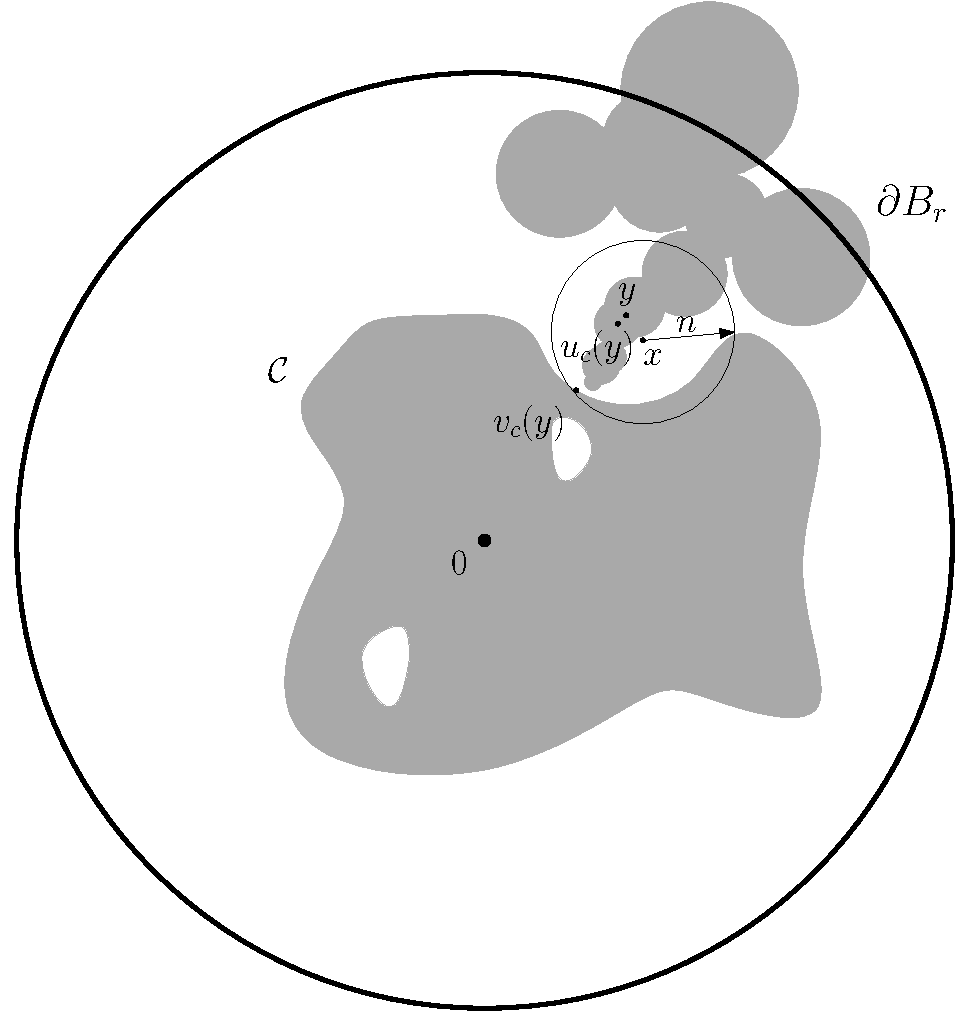
\includegraphics[width=0.60\linewidth]{image.pdf}
\caption{A simultaneous occurrence of the events $ {\mathcal E}_y$, $ {\mathcal F}_y$, $ {\mathcal G}_y$, and $ {\mathcal H}_y$. }\label{fig:aaa}
\end{figure}

Now, observe that if ${\mathcal E}_y$ and ${\mathcal H}_y$ occur simultaneously, then ${\mathcal P}_x(n)$ occurs (we use ${\rbf^*}\ge \sqrt d$). Furthermore if ${\mathcal F}_y$ and ${\mathcal G}_y$ also occur simultaneously with them, then $\mathsf B^{v_{\Cbf}}_{\rbf^*}\cap{\Cbf}'\ne \emptyset$. Since by construction $v_{\Cbf}\in \mathsf B^x_{3n}$, we deduce that $d({\Cbf}\cap\mathsf B^x_{3n},{\Cbf}')<{\rbf^*}$. Integrating~\eqref{eq:r} on ${\mathcal E}_y$, we deduce that
\[
{\mathbb P}_\lambda[{\mathcal P}_x(n)\text{ and }d({\Cbf}\cap\mathsf B^x_{3n},{\Cbf}')<{\rbf^*}]\ge{\mathbb P}_\lambda[{\mathcal E}_y\cap{\mathcal F}_y\cap{\mathcal G}_y\cap{\mathcal H}_y]\ge \frac{{c_{\IT}}\, c_4}{n^{2d-2}}\,{\mathbb P}_\lambda[{\mathcal E}_y\cap{\mathcal H}_y].
\]
Observe that if ${\mathcal P}_x(n)$ and $d({\Cbf}\cap\mathsf B^x_{n},{\Cbf}')\ge {\rbf^*}$ occur, then there exists $y\in {\mathbb Z}^d$ such that the event on the right-hand side occurs. In particular, $\mathsf S^y$ must intersect $\mathsf B^x_{n}$ for ${\mathcal H}_y$ to occur, so that there are $c_6n^d$ possible values for $y$. Summing over all these values, we therefore get that
\[
c_6 n^d\,{\mathbb P}_\lambda[{\mathcal P}_x(n)\text{ and }d({\Cbf}\cap\mathsf B^x_{3n},{\Cbf}')< {\rbf^*}]\ge \frac{{c_{\IT}}\, c_4}{n^{2d-2}}\,{\mathbb P}_\lambda[{\mathcal P}_x(n)\text{ and }d({\Cbf}\cap\mathsf B^x_{n},{\Cbf}')\ge {\rbf^*}],
\]
which implies the claim~\ref{claim310} readily.
\end{proof}


\section{Renormalization of crossing probabilities}\label{sec:renorm-ofcr-prob}
In this section, we prove Theorems~\ref{thm:2} and~\ref{thm:3}. The proof is quite different in the regime where $\mu[r,\infty]$ decays exponentially fast (light tail), and in the regime where it does not (heavy tail). Also, since in the heavy tail regime the renormalization argument performed below may be of some use in the study of other models, or for different distributions $\mu$, we prove a quantitative lemma which we believe to be of independent interest.

In this section, we reboot the count for the constants $c_i$ starting from $c_1$. The section is organized as follows. In Section~\ref{sec:4.1}, we prove a renormalization lemma, Lemma~\ref{lem:17} which will enable us to derive the theorems. In Sections~\ref{sec:4.2} and~\ref{sec:4.3}, we derive Theorem~\ref{thm:2} and Theorem~\ref{thm:3} respectively.

\subsection{The renormalization lemma}\label{sec:4.1}

Introduce, for every $\delta,\alpha,\lambda\ge0$ and $r\ge1$, the two functions
\begin{align*}
\pi_r^\delta(\lambda)&:={\mathbb P}_\lambda[\exists (z,R)\in\eta\text{ such that } \mathsf B_R^z \cap \mathsf B_{2\delta r}\ne \emptyset\text{ and }\mathsf B_R^z \cap \partial \mathsf B_{(1-2\delta)r}\ne \emptyset],\\
\theta_r^\alpha(\lambda) &:= {\mathbb P}_{\lambda} [\mathsf B_{\alpha r} \longleftrightarrow \partial \mathsf B_r].
\end{align*}
Note that $\pi_r^0(\lambda)=\phi_r(\lambda)$ and $\theta_r^0(\lambda)=\theta_r(\lambda)$ by definition.

\begin{rema}
The quantity $\pi_r^\delta(\lambda)$ is expressed in terms of $\mu$ as follows: let $c_d$ be the area of the sphere of radius 1 in ${\mathbb R}^d$, then
\begin{equation}\label{eq:p1}
\pi_r^\delta(\lambda)=1-\exp\Big(-\lambda c_d \int_0^\infty a^{d-1}\mu[|a-2\delta r|\vee |r-2\delta r-a|,\infty]da\Big).
\end{equation}
\end{rema}

The following Lemma~\ref{lem:17} will be the key to the proofs of the Theorems~\ref{thm:2} and~\ref{thm:3}.
\begin{lemm}[Renormalization inequality]\label{lem:17}
For every $0<\alpha\le \delta\le 1/4$, there exists $c_1>0$ such that for every $\lambda,r>0$,
\begin{equation}\label{eq:14}
\theta^\alpha_r (\lambda)\le \pi_r^\delta(\lambda)+\frac{c_1}{(\delta^2\alpha)^d}\,\max_{\substack{u,v\ge\delta \\ u+v=1-\alpha}}\theta^\alpha_{ur}(\lambda)\,\theta^\alpha_{vr}(\lambda).
\end{equation}
\end{lemm}

Note that the smaller the $\alpha$ and $\delta$, the larger the entropic factor $c_1/(\delta^2\alpha)^d$. We will see that the choices of $\alpha$ and $\delta$ are important in the applications. Except for the exponential bound on $\theta_r(\lambda)$ in the proof of Theorem~\ref{thm:2}, we will always pick $\delta=\alpha$.
\begin{proof}
Fix $0<\alpha\le \delta\le 1/4$ and $\lambda,r>0$. Set
\[
E:=\{2\delta r\}\cup \left([2\delta r,(1-2\delta)r]\cap \tfrac{\alpha\delta}{2} r{\mathbb Z}\right)\cup\{(1-2\delta)r\}
\]
and index the elements of $E$ in the increasing order by $r_0< r_1<\dots< r_\ell$. Recall the notation $\eta^Z$ for the set of $(z,R)\in \eta$ with $\mathsf B_R^z\subset Z$, and introduce the three events
\begin{align*}
{\mathcal A}&:=\left\{\exists (z,R)\in\eta:\mathsf B_R^z\cap\mathsf B_{2\delta r}\ne\emptyset\text{ and }\mathsf B_R^z\cap\partial\mathsf B_{(1-2\delta) r}\ne\emptyset\right\},\\
{\mathcal B}_k&:=\left\{\mathsf B_{\alpha r}\longleftrightarrow\partial\mathsf B_{r_k}\text{ in }{\mathcal O}\left(\eta^{\mathsf B_{r_{k+1}}}\right)\right\},\\
{\mathcal C}_k&:=\left\{\mathsf B_{r_{k+1}}\longleftrightarrow\partial\mathsf B_{r}\right\}.
\end{align*}
If $\mathsf B_{\alpha r}$ is connected to $\partial\mathsf B_r$ but ${\mathcal A}$ does not occur, then ${\mathcal B}_k\cap{\mathcal C}_k$ must occur for some $0\le k<\ell$ (we use that $\delta\ge\alpha$). Furthermore, by construction, ${\mathcal B}_k$ and ${\mathcal C}_k$ are independent since ${\mathcal C}_k$ is measurable with respect to ${\mathcal O}(\eta\setminus\eta^{\mathsf B_{r_{k}}})$. These two observations together imply that
\begin{align}\label{eq:j1}
\theta^\alpha_r (\lambda)&\le {\mathbb P}_\lambda[{\mathcal A}]+\sum_{k=0}^{\ell-1}{\mathbb P}_\lambda[{\mathcal B}_k\cap{\mathcal C}_k]=\pi^\delta_r(\lambda)+\sum_{k=0}^{\ell-1}{\mathbb P}_\lambda[{\mathcal B}_k]{\mathbb P}_\lambda[{\mathcal C}_k].
\end{align}
Fix $0\le k < \ell$. Let $X$ denote a set of points $x\in\partial\mathsf B_{\alpha r}$ such that the union of the balls $\mathsf B_{\alpha \delta r}^x$ for $x\in X$ covers $\partial\mathsf B_{\alpha r}$. Choose $X$ such that $|X|\le c_2 \delta^{-(d-1)}$. Applying the union bound, we find
\begin{align}
{\mathbb P}_\lambda[{\mathcal B}_k]&\le \sum_{x\in X}{\mathbb P}_\lambda\left[\mathsf B_{\alpha \delta r}^x\longleftrightarrow \partial\mathsf B_{r_k-\alpha r}^x\right]\le|X|\,\theta_{r_k-\alpha r}^\alpha(\lambda)\le \frac {c_2}{\delta^{d-1}}\,\theta_{r_k-\alpha r}^\alpha(\lambda).\label{eq:12}
\end{align}
Similarly, using a covering of $\partial\mathsf B_{r_{k+1}}$ with at most $c_2'(\alpha\delta)^{1-d}$ balls of radius $\alpha\delta r$ centered on $\partial \mathsf B_{r_k}$, we obtain
\begin{equation}\label{eq:11}
{\mathbb P}_\lambda[{\mathcal C}_k]\le \frac{c_2'}{(\delta\alpha)^{d-1}} \,\theta_{r-r_k}^\alpha(\lambda).
\end{equation}
Plugging~\eqref{eq:12} and~\eqref{eq:11} in~\eqref{eq:j1} and using the fact that $\ell\le 2/(\alpha\delta)$ concludes the proof of Lemma~\ref{lem:17}.
\end{proof}

The previous Lemma~\ref{lem:17} leads to Proposition~\ref{cor:a}.


\begin{proof}[Proof of Proposition~\ref{cor:a}]
Choose $\alpha=1/6$. In this case
\[
\theta_{r}^\alpha(\lambda)={\mathbb P}_\lambda[\mathsf B_{r/6}\longleftrightarrow\partial\mathsf B_{r}].
\]
Using a covering of $\partial\mathsf B_r$ with balls of radius $r/6$, it suffices to prove that $\theta_{r}^\alpha(\lambda)$ converges to $0$. A reasoning similar to the bound on ${\mathbb P}_\lambda[{\mathcal B}_k]$ in the last proof implies that for every $s\in[\alpha r, r]$,
\begin{equation}
\theta_r^\alpha(\lambda)\le c_3\,\theta_s^\alpha(\lambda),\label{eq:l1}
\end{equation}
which enables us to rewrite~\eqref{eq:14} (applied with $\delta=\alpha=1/6$) as
\[
\theta_r^\alpha(\lambda)\le \pi^{\alpha}_r(\lambda)+c_4 \,\theta^\alpha_{\alpha r}(\lambda)^2.
\]
Now, fix $\ep>0$ such that $2c_4\ep<1$ and work with $r_0$ large enough that $\pi^{\alpha}_r(\lambda)\le \ep/2$ for every $r\ge r_0$.

Now, assume that there exists $r\ge r_0$ such that $\theta_r^\alpha(\lambda)<\ep$. We deduce inductively that
\[
\theta_{r/\alpha^k}^\alpha(\lambda)\le \ep
\]
for every $k\ge1$.
Using~\eqref{eq:l1} one last time gives that $\theta_s^\alpha(\lambda)\le c_3\ep$ for every $s\ge r$.

We conclude that for every $\lambda<\widetilde \lambda_c$, ${\mathbb P}_\lambda[\mathsf B_r\longleftrightarrow\partial\mathsf B_{2r}]$ tends to 0. Since the set of $\lambda$ such that there exists $r$ with $\theta_r^\alpha(\lambda)<\ep$ is open, we deduce that every $\lambda\ge\widetilde\lambda_c$, $\theta_r^\alpha(\lambda)\ge\ep$.
\end{proof}

\begin{rema}\label{rmk:finite}
Fix $\alpha=\tfrac16$ and consider $r_1$ such that $7c_4\theta_r^\alpha(\lambda)<1$ for every $r\ge r_1$, where $c_4$ is given by~\eqref{eq:l1}. Consider the quantity $S_R(\lambda):=\int_{0}^R r^{d-1}\theta^\alpha_r(\lambda)dr$. Integrating~\eqref{eq:l1}, we find that
\[
S_R(\lambda)\le r_1+\int_{r_1}^Rr^{d-1}\pi^\alpha_r(\lambda)dr +\tfrac67S_{R/6}(\lambda),
\]
which easily implies, using the assumption~\eqref{eq:5} that $\sup\{S_R(\lambda):R\ge1\}<\infty$. Now, we have that the expected size of the origin is bounded by this supremum, and is therefore also finite.
\end{rema}

\subsection{Proof of Theorem~\ref{thm:2}}\label{sec:4.2}


Consider $\lambda<\widetilde \lambda_c$. Fix $\delta\in(0,\tfrac12)$ and observe that since $\mu[r,\infty]\le \exp(-cr)$, \eqref{eq:p1} implies that there exists $c'>0$ such that $\pi_r^\delta(\lambda)\le \exp(-c' r)$ for every $r\ge1$. We now proceed in two steps: we first show that $\theta_r(\lambda)\le r^{-d-1}$ for $r$ large enough, and then improve this estimate to an exponential decay.

\subsection{Polynomial bound on $\theta_r(\lambda)$}
Lemma~\ref{lem:17} applied to $\alpha=\delta=1/6$ implies that for every $r\ge 1$
\begin{equation}\label{eq:6}
\theta_r^\alpha(\lambda) \le e^{-c' r}+c_5 \max_{\substack{u,v\ge\alpha \\ u+v=1-\alpha}}\theta_{ur}^\alpha(\lambda)\theta_{vr}^\alpha(\lambda).
\end{equation}
Since $\lambda<\widetilde \lambda_c$, Proposition~\ref{cor:a} implies that $\theta_r^\alpha(\lambda)$ converges to $0$ as $r$ tends to infinity. In particular, we deduce that for every $\ep>0$,
\[
\theta_r^\alpha(\lambda)\le e^{-c' r}+\ep\,\theta_{\alpha r}^\alpha(\lambda)
\]
for $r$ large enough. A simple induction implies that $\theta_r^\alpha(\lambda)\le r^{-d-1}$ for $r$ large enough.


\subsection{Exponential bound on $\theta_r(\lambda)$}
Choose $\delta=1/6$. For each $r\ge6$, apply Lemma~\ref{lem:17} with $\alpha=\alpha(r):=1/r$ to get that
\[
\theta_r(\lambda)\le e^{-c'r}+c_6r^d \max_{\substack{u,v\ge\tfrac16 \\ u+v=1-\alpha(r)}}\theta_{ur}(\lambda)\theta_{vr}(\lambda),
\]
where we use that
\[
\theta_r(\lambda)\le \theta_r^{\alpha(r)}(\lambda)={\mathbb P}_\lambda[\mathsf B_1\longleftrightarrow\partial\mathsf B_r]\le \tfrac1{c_{\IT}}\theta_r(\lambda).
\]
Set $c_7:=2 \, c_6 \, e $ and consider $r_0$ large enough so that for every $r\ge \delta r_0$,
\begin{align*}
&c_7r^d\,e^{-c'r}\le \tfrac12e^{-r/r_0},\text{ and }\\
&c_7r^d\,\theta_r(\lambda)\le e^{-1}.
\end{align*}
(The second constraint is satisfied thanks to the polynomial bound derived in the first part of the proof.) By induction on $k$, one can show that for every $k\ge 0$,
\[
\forall r\in[\delta r_0, r_0/(1-\delta)^k]\quad c_7r^d\,\theta_r(\lambda)\le \exp(-r/r_0).
\]

\subsection{Proof of Theorem~\ref{thm:3}}\label{sec:4.3}

In this section, we prove Theorem~\ref{thm:3} by proving the following quantitative Lemma~\ref{thm:16}. We believe the lemma to be of value for distributions $\mu$ other than the one considered in Theorem~\ref{thm:3}. Before that, note that the lower bound
\begin{equation}
\theta_r(\lambda)\ge \phi_r(\lambda)\label{eq:m1}
\end{equation}
for every $r>0$ is trivial since 0 is connected to $\partial\mathsf B_r$ in the case where there exists $(z,R)\in \eta$ such that $\mathsf B_R^z$ contains 0 and intersects $\partial\mathsf B_r$. Therefore, the main concern of this section will be an upper bound on $\theta_r^\alpha(\lambda)$ (which is larger than $\theta_r(\lambda)$).

\begin{lemm}\label{thm:16}
Consider $\lambda>0$, $\eta<1$ and $\alpha\in(0,\tfrac14)$ small enough such that $\alpha^{\eta}+(1-2\alpha)^{\eta}\ge 1$. For every $\ep>0$ sufficiently small and $r\ge1$, if there exists $r_0\le \alpha r$ such that
\begin{align}
\theta_s^\alpha(\lambda)&\le \ep\, \pi_{r}^\alpha(\lambda)^{(s/r)^\eta}\quad\forall s\in[r_0,r_0/\alpha]\label{eq:f1}
\\
\pi_s^\alpha(\lambda)&\le \ep\,\pi_r^\alpha(\lambda)^{(s/r)^\eta}\quad\forall s\in[r_0,(1-\alpha)r],\label{eq:f2}
\end{align}
then
\begin{equation}
\theta_{r}^\alpha(\lambda)\le (1+\ep)\,\pi_{r}^\alpha(\lambda).
\end{equation}
\end{lemm}

\begin{rema}\label{rem:22}\ \\*[-1.6em]
\begin{enumerate}
\item Note that distributions $\mu$ with exponential decay do not satisfy the assumptions of the lemma for any $r$, provided that $\ep$ is small enough. %%\medbreak
\item For distributions $\mu$ satisfying $\lim_{r\rightarrow\infty}\pi_r^\alpha(\lambda)^{1/r^\eta}= \kappa$, for some constant $\kappa$, the existence of $r_0$ satisfying~\eqref{eq:f1} when $\lambda<\tilde\lambda_c$ follows directly from
\begin{itemize}%%[noitemsep,nolistsep]
\item picking $r_0$ such that $\theta_r^\alpha(\lambda)<\tfrac{\ep}{2\kappa}$ for every $r\ge r_0$ (by Proposition~\ref{cor:a}),
\item picking $r$ large enough that $\pi_r^\alpha(\lambda)^{1/r^\eta}\ge \kappa 2^{-(\alpha/r_0)^\eta}$.
\end{itemize}
\item The second assumption~\eqref{eq:f2} is a regularity statement on $\pi_r^\alpha(\lambda)$ that can be obtained from the regularity of $\mu[r,\infty]$ using~\eqref{eq:p1}.
\end{enumerate}
\end{rema}


The proof of the Lemma~\ref{thm:16} will be based on the recursive relation given by Lemma~\ref{lem:17}. We use a strategy which is inspired by the study of differential equations. We control the function $f(s):=\theta_s^\alpha(\lambda)$ in terms of $g(s):=\pi_r^\alpha(\lambda)^{(s/r)^\eta}$ uniformly for $s\in [r_0, (1-\alpha) r]$ to finally deduce a bound for $f(r)$ using again Lemma~\ref{lem:17}.

\begin{proof}
Set $C=c_1\alpha^{-2d}$, where $c_1$ is given by Lemma~\ref{lem:17}, and assume that $\ep<\tfrac1{4C}$. The key ingredient will be the following inequality: for every $s\in[r_0,(1-\alpha)r]$,
\begin{equation}\label{eq:h1}
\theta_s^\alpha(\lambda)\le 2\ep\, \pi_r^\alpha(\lambda)^{(s/r)^\eta}.
\end{equation}
For $s\in[r_0,r_0/\alpha]$, \eqref{eq:h1} follows from~\eqref{eq:f1}. To obtain the claim for $s> r_0/\alpha$, use the induction hypothesis in the second line below to get
\begin{align*}
\theta^\alpha_s(\lambda)&\stackrel{{\eqref{eq:14}}}\le \pi_s^\alpha(\lambda)~+~C \max_{\substack{u,v\ge \alpha \\ u+v=1-\alpha}}\theta^\alpha_{us}(\lambda)\,\theta^\alpha_{vs}(\lambda)\\
&\stackrel{\eqref{eq:h1}}\le \pi_s^\alpha(\lambda)~+~4C\ep^2 \max_{\substack{u,v\ge\alpha \\ u+v=1-\alpha}}\pi^\alpha_r(\lambda)^{(u^\eta+v^\eta)(s/r)^\eta}\\
&\stackrel{\eqref{eq:f2}}\le \left(\ep+4C\ep^2\right)\, \pi_r^\alpha(\lambda)^{(s/r)^\eta}\\
&\stackrel{\phantom{\eqref{eq:f2}}}\le 2\ep\,\pi_r^\alpha(\lambda)^{(s/r)^\eta}.
\end{align*}
In the first line, we applied~\eqref{eq:14} with $\delta=\alpha$. In the second line, we used~\eqref{eq:h1} for $us,vs\in[r_0,s-r_0]$ and in the third line we used $u^\eta+v^\eta\ge 1$ for every $u,v\ge\alpha$ satisfying $u+v=1-\alpha$. One may apply the first two lines in the previous sequence of inequalities for $s=r$ (since in such case $ur,vr\in[r_0,(1-\alpha)r]$) so that
\begin{align*}
\theta^\alpha_r(\lambda)&
\le \pi_r^\alpha(\lambda)+4C\ep^2 \max_{\substack{u,v\ge\alpha \\ u+v=1-\alpha}}\pi^\alpha_r(\lambda)^{u^\eta+v^\eta}\le (1+\ep)\, \pi_r^\alpha(\lambda).
\end{align*}
This concludes the proof of the Lemma~\ref{thm:16}.
\end{proof}


\begin{proof}[Proof of Theorem~\ref{thm:3}]
Fix $\lambda<\widetilde\lambda_c$.
Since~\eqref{eq:m1} gives the lower bound, we focus on the upper bound. Under the condition~\eqref{C1}, define $f(\alpha,r)$ by
\begin{equation}\label{eq:n1}
\pi_r^\alpha(\lambda)=f(\alpha,r) r^{-c},
\end{equation}
and, under the condition~\eqref{C2}, define $g(\alpha,r)$ by
\begin{equation}\label{eq:n2}
\pi_r^\alpha(\lambda)=g(\alpha,r) r^{d-\gamma} \exp\left[-c \left(\frac r 2-{2\alpha} r\right)^\gamma\right]. 
\end{equation}
Using~\eqref{eq:p1}, one can check that $f(\alpha,r)$ and $g(\alpha,r)$ converge (as $r$ tends to infinity) uniformly in $0\le \alpha<\tfrac14$ to two continuous positive functions $f(\alpha)$ and $g(\alpha)$.

Consider $\ep$ very small and use Proposition~\ref{cor:a} to guarantee that $\theta_{s}^\alpha(\lambda)<\ep$ for every $s$ large enough. Then, for every distribution $\mu$ satisfying~\eqref{C1}  or~\eqref{C2}, one can find $0<\eta<1$, $r_0$ large enough such that~\eqref{eq:f1} and~\eqref{eq:f2} are satisfied for every $r\ge r_0$ large enough, and $\alpha$ small enough (use~\eqref{eq:n1} and~\eqref{eq:n2} and Remark~\ref{rem:22} to check the two conditions), so that Lemma~\ref{thm:16} implies that for $r$ large enough,
\begin{equation}
\theta_r^\alpha(\lambda)\le (1+\ep)\pi_r^\alpha(\lambda)\label{eq:bn}
.
\end{equation}

Thanks to~\eqref{eq:n1}, we obtain the claim in case~\eqref{C1} by letting $\ep$ and then $\alpha$ tend to 0. For case~\eqref{C2}, we need to do more, since letting $\alpha$ tend to 0 slowly gives only that $\theta_r(\lambda)\le \phi_r(\lambda)^{1+o(1)}$. More precisely, we prove the following claim.

\begin{enonce}[plain]{Claim}\label{claim4.6}
Assume that $\mu$ satisfies $\eqref{C2}$. Fix $\overline \gamma\in(\gamma,1)$. There exist $\alpha>0$ and $R<\infty$ such that for every $k\ge0$ and every $r\ge 3^kR$, we have that
\begin{equation}\label{eq:b2}
\theta_{r}^{\alpha_k}(\lambda)\le (1+2^{-k})\pi_r^{\alpha_k}(\lambda)
\end{equation}
where $\alpha_k:= \alpha 3^{-k \overline\gamma}$.
\end{enonce}


Before proving the Claim~\ref{claim4.6}, note that it implies, together with~\eqref{eq:n2}, that for every $k\ge0$ and $r\in [3^k R,3^{k+1}R)$,
\[
\theta_r(\lambda)\le\theta_{r}^{\alpha_k}(\lambda)\le (1+2^{-k})\pi_r^{\alpha_k}(\lambda)\le (1+2^{-k}) \frac{g(\alpha_k,r)}{g(0,r)}e^{Cr^{\gamma-\overline\gamma}} \phi_r(\lambda)
\]
for some constant $C=C(\alpha,R)>0$. This proves the Theorem~\ref{thm:3} in case~\eqref{C2} thanks to the choice of $\overline\gamma>\gamma$ and the uniform convergence of $g(.\,,r)$ towards a continuous function.
\end{proof}



\begin{proof}[{Proof of the Claim~\ref{claim4.6}}]
We prove~\eqref{eq:b2} recursively. Fix $0< \alpha\le 1/8$ such that
\begin{align}
&2 (1-12\alpha)^\gamma \left(\tfrac{1-\alpha}2\right)^\gamma\ge 1+\tfrac14 \alpha^\gamma,\text{ and} \label{eq:9}
\\\label{eq:10}
&\forall x\in[0,\alpha] \quad (1 - 12x)^{2\gamma}+(x/2)^\gamma
\ge 1+\tfrac14 x^\gamma.
\end{align}
Fix also $R\ge1$. There will be several conditions on $R$ that will be added during the proof. The important feature is that every time a new condition is added, one only needs to take $R$ possibly larger than before.

Define $M$ such that for every $x\le \tfrac14$, $\tfrac2M\le g(x)\le\tfrac M2$. By uniform convergence, $R$ can be chosen large enough that for every $x\le \tfrac14$ and $r\ge R$,
\begin{equation}
\tfrac1M\le g(x,r)\le M.\label{eq:b1}
\end{equation}

Use~\eqref{eq:bn} to choose $R$ in such a way that $\theta_r^{\alpha}(\lambda)\le 2\pi_r^\alpha(\lambda)$ for every $r\ge \alpha R$. Then, \eqref{eq:b2} follows for $k=0$ by definition. We now assume that~\eqref{eq:b2} is valid for $k-1$ and prove it for $k$. Lemma~\ref{lem:17} applied to $r\ge R2^k$ and $\alpha_k$ gives that
\begin{align}\label{eq:c1}
\theta_{r}^{\alpha_k}(\lambda)&\le \pi_{r}^{\alpha_k}(\lambda)+\frac{c_1}{\alpha_k^{3d}} \,\theta_{ur}^{\alpha_k}(\lambda)\,\theta_{vr}^{\alpha_k}(\lambda),
\end{align}
for some $u,v \ge\alpha_k$ such that $u+v=1-\alpha_k$. Without loss of generality, we can assume that $u \geq \frac 1 3$ and $v\le \frac{1-\alpha_k}2$. In particular, we have $ur\ge R3^{k-1}$. Also, $vr\ge \alpha R3^{k (1-\overline\gamma)}\ge \alpha R$. The induction hypothesis (in fact we simply bound $2^{-{(k-1)}}$ by $1$) implies that
\[
\theta_{ur}^{\alpha_k}(\lambda)\le \theta_{ur}^{\alpha_{k-1}}(\lambda)\le 2\pi_{ur}^{\alpha_{k-1}}(\lambda)\quad \text{and}\quad\theta_{vr}^{\alpha_k}(\lambda)\le \theta_{vr}^{\alpha}(\lambda)\le 2\pi_{vr}^\alpha(\lambda).
\]
We may use the induction hypothesis to get that
\begin{align}
\theta_{ur}^{\alpha_k}(\lambda)\theta_{vr}^{\alpha_k}(\lambda)&\stackrel{\eqref{eq:b2}}\le 4 \pi_{ur}^{\alpha_{k-1}}(\lambda)\pi_{vr}^\alpha(\lambda)\nonumber\\
& \stackrel{\eqref{eq:b1}}\leq 4 M^2 (uvr^2)^{d-\gamma} \exp \big[-c(r/2)^\gamma \big((u - 4\alpha_{k-1}u)^\gamma+(v -4 \alpha v)^\gamma\big)\big] \label{eq:8}
.
\end{align}
We now bound the term
\[
h(v):=(u - 4\alpha_{k-1}u)^\gamma+(v -4 \alpha v)^\gamma{=} (1 - 4\cdot 3^{\overline\gamma}\alpha_{k})^\gamma(1-\alpha_k-v)^\gamma+(1-4 \alpha)^\gamma v^\gamma
\]
appearing in the exponential in~\eqref{eq:8}. Since $\alpha_k\le v\le \frac{1-\alpha_k}2$, an elementary analysis of the function $h$ shows that $h(v) \ge \min (h(\alpha_k),h(\tfrac{1-\alpha_k}2))$. Using~\eqref{eq:9} and~\eqref{eq:10} to bound $h(\frac{1-\alpha_k}2)$ and $h(\alpha_k)$ respectively, we obtain
\begin{align*}
h(v)\ge 1+ \tfrac14 \alpha_k^\gamma \ge(1 - 4\alpha_k)^\gamma +\tfrac14 \alpha_k^\gamma.
\end{align*}
Plugging this estimate in~\eqref{eq:8} and using~\eqref{eq:b1} one last time, we finally get
\begin{align*}
\theta_{ur}^{\alpha_k}(\lambda)\theta_{vr}^{\alpha_k}(\lambda)& \stackrel{\phantom{\eqref{eq:b3}}}\leq 4M^3 r^{2d} \exp \left[-\tfrac c8 (\alpha_kr)^\gamma\right] \, \pi_r^{\alpha_k} (\lambda)\\
&\stackrel{\eqref{eq:b3}}\le \frac{\alpha_k^{3d}}{c_12^k}\,\pi_r^{\alpha_k}(\lambda),
\end{align*}
which concludes the proof using~\eqref{eq:c1}. In the second line, we used that $R$ is chosen so large that for every $k\ge0$ and $r\ge 3^k R$,
\begin{equation}\label{eq:b3}
\frac {c_1 2^k}{\alpha_k^{3d}} 4 M^3 r^{2d} \exp \left[-\tfrac c8(\alpha_kr)^\gamma\right] \leq \frac {c_1}{\alpha^{3d}} 4 M^3 r^{6d} \exp \left[-\tfrac c8 (\alpha r^{1-\overline\gamma})^\gamma\right] \leq 1.\qedhere
\end{equation}
\end{proof}\let\qed\relax


\begin{rema}
By adapting the reasoning above, one can prove similar statements for other distributions $\mu$ having sub-exponential tails, for instance $\mu[r,\infty]$ decaying like $\exp[-c(\log r)^\gamma]$ or $\exp[-cr/(\log r)^\gamma]$.
\end{rema}



\begin{thebibliography}{99}
\bibitem{AizBar87}Aizenman, Michael; Barsky, David J. Sharpness of the phase transition in percolation models, Commun. Math. Phys., Volume 108 (1987) no. 3, pp. 489-526 | DOI | Zbl | MR
\bibitem{AizBarFer87}Aizenman, Michael; Barsky, David J.; Fernández, Roberto The phase transition in a general class of Ising-type models is sharp, J. Statist. Phys., Volume 47 (1987) no. 3-4, pp. 343-374 | DOI | MR
\bibitem{ahlberg2016sharpness}Ahlberg, Daniel; Tassion, Vincent; Teixeira, Augusto Sharpness of the phase transition for continuum percolation in $\mathbb{R}^2$ (2016) (https://arxiv.org/abs/1605.05926) | Zbl
\bibitem{ATT17}Ahlberg, Daniel; Tassion, Vincent; Teixeira, Augusto Existence of an unbounded vacant set for subcritical continuum percolation (2017) (https://arxiv.org/abs/1706.03053) | Zbl
\bibitem{BefDum12}Beffara, Vincent; Duminil-Copin, Hugo The self-dual point of the two-dimensional random-cluster model is critical for $q\ge 1$, Probab. Theory Related Fields, Volume 153 (2012) no. 3-4, pp. 511-542 | DOI | Zbl | MR
\bibitem{BroHam57}Broadbent, S. R.; Hammersley, John M. Percolation processes. I. Crystals and mazes, Proc. Cambridge Philos. Soc., Volume 53 (1957), pp. 629-641 | DOI | Zbl | MR
\bibitem{BolRio06}Bollobás, Béla; Riordan, Olivier The critical probability for random Voronoi percolation in the plane is 1/2, Probab. Theory Related Fields, Volume 136 (2006) no. 3, pp. 417-468 | DOI | Zbl | MR
\bibitem{GRSY18}Duminil-Copin, Hugo; Goswami, Subhajit; Raoufi, Aran; Severo, Franco; Yadin, Ariel Existence of phase transition for percolation using the Gaussian Free Field (2018) (https://arxiv.org/abs/1806.07733)
\bibitem{DGRS19}Duminil-Copin, Hugo; Goswami, Subhajit; Rodriguez, P.-F.; Severo, Franco Equality of critical parameters for GFF level-set percolation (2019) (in preparation)
\bibitem{DumRaoTas16b}Duminil-Copin, Hugo; Raoufi, Aran; Tassion, Vincent Exponential decay of connection probabilities for subcritical Voronoi percolation in $\mathbb{R}^d$ (2017) (https://arxiv.org/abs/1705.07978, to appear in Probab. Theory Related Fields) | Zbl
\bibitem{DumRaoTas16a}Duminil-Copin, Hugo; Raoufi, Aran; Tassion, Vincent Sharp phase transition for the random-cluster and Potts models via decision trees (2017) (https://arxiv.org/abs/1705.03104) | Zbl
\bibitem{DumTas15}Duminil-Copin, Hugo; Tassion, Vincent A new proof of the sharpness of the phase transition for Bernoulli percolation and the Ising model, Commun. Math. Phys., Volume 343 (2016) no. 2, pp. 725-745 | DOI | Zbl | MR
\bibitem{Gil}Gilbert, Edgar N. Random plane networks, J. Soc. Indust. Appl. Math., Volume 9 (1961), pp. 533-543 | DOI | MR
\bibitem{Gou1}Gouéré, Jean-Baptiste Subcritical regimes in the Poisson Boolean model of continuum percolation, Ann. Probab., Volume 36 (2008) no. 4, pp. 1209-1220 | DOI | Zbl | MR
\bibitem{Gou2}Gouéré, Jean-Baptiste; Théret, Marie Equivalence of some subcritical properties in continuum percolation (2018) (https://arxiv.org/abs/1803.00793) | Zbl
\bibitem{Hal}Hall, Peter On continuum percolation, Ann. Probab., Volume 13 (1985) no. 4, pp. 1250-1266 | DOI | Zbl | MR
\bibitem{LP17}Last, Günter; Penrose, Mathew D.x Lectures on the Poisson process, Institute of Mathematical Statistics Textbooks, 7, Cambridge University Press, 2017 | Zbl
\bibitem{Men86}Menshikov, Mikhail V. Coincidence of critical points in percolation problems, Dokl. Akad. Nauk SSSR, Volume 288 (1986) no. 6, pp. 1308-1311 | MR
\bibitem{MeeRoy08}Meester, Ronald; Roy, Rahul Continuum percolation, Cambridge University Press, 1996 | Zbl
\bibitem{meester1994nonuniversality}Meester, Ronald; Roy, Rahul; Sarkar, Anish Nonuniversality and continuity of the critical covered volume fraction in continuum percolation, J. Statist. Phys., Volume 75 (1994) no. 1-2, pp. 123-134 | DOI | Zbl | MR
\bibitem{OSSS}O’Donnell, Ryan; Saks, Mickael E.; Schramm, O.; Servedio, Rocco A. Every decision tree has an influential variable, 2019 IEEE 60th Annual Symposium on Foundations of Computer Science (FOCS), IEEE Xplore (2005), pp. 31-39
\bibitem{Pen17}Penrose, Mathew D. Non-triviality of the vacancy phase transition for the Boolean model (2017) (https://arxiv.org/abs/1706.02197) | Zbl
\bibitem{Zie16}Ziesche, Sebastian Sharpness of the phase transition and lower bounds for the critical intensity in continuum percolation on $\mathbb{R}^d$ (2016) (https://arxiv.org/abs/1607.06211, to appear in Annales de l’Institut Henri Poincaré) | Zbl
\bibitem{zuev1985continuous}Zuev, Sergei A.; Sidorenko, Alexander Continuous models of percolation theory. I, Teor. Mat. Fiz., Volume 62 (1985) no. 2, pp. 51-58 | DOI
\end{thebibliography}
\end{document}
